%\usetikzlibrary{backgrounds} % DEBUG
%background rectangle/.style={fill=olive!45}, show background rectangle
\begin{figure}
	\centering
	\begin{minipage}{1.0\textwidth}
		\centering
		\begin{tikzpicture}[scale=1, trim axis left, trim axis right]
			\begin{axis}[xlabel=$t$, ylabel={$\langle\hat{\sigma}_z\rangle$}, grid=both, grid style={gray!20}, every axis plot/.append style={very thick}, scale only axis, height=\singleFigureHeight, width=\singleFigureWidth, legend style={at={(1.2715,0.9)}, anchor=north west, font=\small, nodes={scale=\legendscale, transform shape}, label={[font=\small]above:{MPS DMRG}}}, legend columns=1, legend cell align={left}, xmin=-0.05, xmax=1.05, ymin=0.78, ymax=1.02]
				%
				\addplot[color = 7blue1]
				table[x=t_tenpy, y=sz_chi_16, col sep=space]{figures/plots/TFI/global_quench/data/global_quench_g_critical_tenpy.txt};
				\addlegendentry{$\chi = 16$}
				%
				\addplot[color = 7blue2]
				table[x=t_tenpy, y=sz_chi_32, col sep=space]{figures/plots/TFI/global_quench/data/global_quench_g_critical_tenpy.txt};
				\addlegendentry{$\chi = 32$}
				%
				\addplot[color = 7blue3]
				table[x=t_tenpy, y=sz_chi_64, col sep=space]{figures/plots/TFI/global_quench/data/global_quench_g_critical_tenpy.txt};
				\addlegendentry{$\chi = 64$}
				%
				\addplot[color = 7blue4]
				table[x=t_tenpy, y=sz_chi_128, col sep=space]{figures/plots/TFI/global_quench/data/global_quench_g_critical_tenpy.txt};
				\addlegendentry{$\chi = 128$}
				%
				\addplot[color = 7blue5]
				table[x=t_tenpy, y=sz_chi_256, col sep=space]{figures/plots/TFI/global_quench/data/global_quench_g_critical_tenpy.txt};
				\addlegendentry{$\chi = 256$}
				%
				\addplot[color = 7blue6]
				table[x=t_tenpy, y=sz_chi_512, col sep=space]{figures/plots/TFI/global_quench/data/global_quench_g_critical_tenpy.txt};
				\addlegendentry{$\chi = 512$}
				%
				\addplot[color = 7blue7]
				table[x=t_tenpy, y=sz_chi_1024, col sep=space]{figures/plots/TFI/global_quench/data/global_quench_g_critical_tenpy.txt};
				\addlegendentry{$\chi = 1024$}
				%
			\end{axis}
			\begin{axis}[every axis plot/.append style={thick}, scale only axis, height=\singleFigureHeight, width=\singleFigureWidth, legend style={at={(1.015,0.9)}, anchor=north west, font=\small, nodes={scale=\legendscale, transform shape}, label={[font=\small]above:{disoTPS}}}, legend columns=1, clip mode=individual, legend cell align={left}, yticklabels=\empty, xmin=-0.05, xmax=1.05, ymin=0.78, ymax=1.02]
				%
				\addplot[color = 5red1]
				table[x=t_disoTPS, y=sz_disoTPS_D_2, col sep=space]{figures/plots/TFI/global_quench/data/global_quench_g_critical_disoTPS.txt};
				\addlegendentry{$D = 2$}
				%
				\addplot[color = 5red2]
				table[x=t_disoTPS, y=sz_disoTPS_D_3, col sep=space]{figures/plots/TFI/global_quench/data/global_quench_g_critical_disoTPS.txt};
				\addlegendentry{$D = 3$}
				%
				\addplot[color = 5red3]
				table[x=t_disoTPS, y=sz_disoTPS_D_4, col sep=space]{figures/plots/TFI/global_quench/data/global_quench_g_critical_disoTPS.txt};
				\addlegendentry{$D = 4$}
				%
				\addplot[color = 5red4]
				table[x=t_disoTPS, y=sz_disoTPS_D_5, col sep=space]{figures/plots/TFI/global_quench/data/global_quench_g_critical_disoTPS.txt};
				\addlegendentry{$D = 5$}
				%
				\addplot[color = 5red5]
				table[x=t_disoTPS, y=sz_disoTPS_D_6, col sep=space]{figures/plots/TFI/global_quench/data/global_quench_g_critical_disoTPS.txt};
				\addlegendentry{$D = 6$}
				%
			\end{axis}%
		\end{tikzpicture}%
	\end{minipage}
	\caption{In this figure we show the time evolution of the $\langle\hat{\sigma}_z\rangle$ expectation value of a spin in the middle of the $8\times8$ diagonal square lattice, containing in total $N = 128$ spins. As a model we use the TFI model at critical field $g_\text{C}$. We compute the time evolution once with DMRG on a MPS and once with disoTPS with the parameters given in the text. We observe good agreement up to times of $t\approx 0.2$, when the two disoTPS results diverge from the DMRG reference simulation.}
	\label{fig:disoTPS_time_evolution_g_critical}
\end{figure}
As a second experiment we study the capabilities of disoTPS to perform real-time evolution. For this we perform a global quench by initializing the disoTPS to a product state, which we then evolve in time, measuring local expectation values. We start with an all-up-state $|\Psi\rangle = |\uparrow\rangle\otimes\cdots\otimes|\uparrow\rangle$ on the square lattice and evolve with the Hamiltonian of the TFI model at critical transverse field $g \approx 3.04438$. At the critical field the entanglement is expected to grow very quickly, making this a hard problem. For the disoTPS we choose bond dimensions of $D\in\left\{2, 3, 4, 5, 6\right\}$, $\chi = 6\cdot D$ and a step size of $\Delta t = 0.02$. We evolve up to time $t = 1.0$, requiring 50 full TEBD iterations. For the YB-move we used approximate TRM disentangling optimizing the Rényi $\alpha = 0.5$ entropy for a maximum number of $N_\text{iter}^\text{YB} = 100$ iterations. For the application of the TEBD bond operators we used a maximum of $N_\text{iters}^\text{bond-op} = 100$ iterations. For a comparison we used the time evolution algorithm from \cite{cite:time_evolving_a_mps_with_long_range_interactions} defined on MPS, which is able to perform time evolution in the presence of long range interactions and is implemented in tenpy \cite{cite:tenpy}. For this reference simulation we used bond dimensions ranging from $\chi = 16$ to $\chi= 1024$ and a time step of $\Delta t = 0.01$. We show the results in figure \figref{fig:disoTPS_time_evolution_g_critical}. We observe that disoTPS is in good agreement with the reference simulation up to a time of $t\approx0.2$, at which the expectation value diverges. This happens at earlier times for smaller bond dimensions $D$. We expect that this fast divergence is due to the accumulated error of the YB move. One could improve the method by applying a per-column variational optimization as done in isoTPS \cite{cite:isometric_tensor_network_states_in_two_dimensions, cite:efficient_simulation_of_dynamics_in_two_dimensional_quantum_spin_systems}, which was found to be essential for real-time evolution \cite{cite:efficient_simulation_of_dynamics_in_two_dimensional_quantum_spin_systems}, or by improving the YB move. \par
%\usetikzlibrary{backgrounds} % DEBUG
%background rectangle/.style={fill=olive!45}, show background rectangle
\begin{figure}
	\centering
	\begin{minipage}[t]{1.0\textwidth}
		\hspace{20pt}
		\begin{tikzpicture}[scale=1, trim axis left, trim axis right]
			\begin{axis}[xlabel=$t$, ylabel=$\langle\hat{\sigma}_z\rangle$, grid=both, grid style={gray!20}, every axis plot/.append style={very thick}, scale only axis, height=\globalQuenchLargeFieldFigureHeight, width=\globalQuenchLargeFieldFigureWidth, xmin=-0.05, xmax=1.05, ymin=-1.1, ymax=1.1, legend style={nodes={scale=\legendscale, transform shape, font=\small}}, legend pos=south east]
				%	
				\addplot[color = 5blue1]
				table[x=t_tenpy, y=sz_chi_16, col sep=space]{figures/plots/TFI/global_quench/data/global_quench_g_6.0_tenpy_site_index_4_4_0.txt};
				\addlegendentry{$\chi= 16$}
				%	
				\addplot[color = 5blue2]
				table[x=t_tenpy, y=sz_chi_32, col sep=space]{figures/plots/TFI/global_quench/data/global_quench_g_6.0_tenpy_site_index_4_4_0.txt};
				\addlegendentry{$\chi= 32$}
				%	
				\addplot[color = 5blue3]
				table[x=t_tenpy, y=sz_chi_64, col sep=space]{figures/plots/TFI/global_quench/data/global_quench_g_6.0_tenpy_site_index_4_4_0.txt};
				\addlegendentry{$\chi= 64$}
				%	
				\addplot[color = 5blue4]
				table[x=t_tenpy, y=sz_chi_128, col sep=space]{figures/plots/TFI/global_quench/data/global_quench_g_6.0_tenpy_site_index_4_4_0.txt};
				\addlegendentry{$\chi= 128$}
				%	
				\addplot[color = 5blue5]
				table[x=t_tenpy, y=sz_chi_256, col sep=space]{figures/plots/TFI/global_quench/data/global_quench_g_6.0_tenpy_site_index_4_4_0.txt};
				\addlegendentry{$\chi= 256$}
				%
			\end{axis}%
			\begin{axis}[scale only axis, height=\globalQuenchLargeFieldFigureHeight, width=\globalQuenchLargeFieldFigureWidth, every axis plot/.append style={very thick}, xmin=-0.05, xmax=1.05, ymin=-1.1, ymax=1.1, legend style={nodes={scale=\legendscale, transform shape, font=\small}}, legend pos=north west]
				%	
				\addplot[color = 3red1]
				table[x=t_disoTPS, y=sz_disoTPS_D_2, col sep=space]{figures/plots/TFI/global_quench/data/global_quench_g_6.0_disoTPS_site_index_4_4_0.txt};
				\addlegendentry{$D = 2$}
				%	
				\addplot[color = 3red2]
				table[x=t_disoTPS, y=sz_disoTPS_D_4, col sep=space]{figures/plots/TFI/global_quench/data/global_quench_g_6.0_disoTPS_site_index_4_4_0.txt};
				\addlegendentry{$D = 4$}
				%	
				\addplot[color = 3red3]
				table[x=t_disoTPS, y=sz_disoTPS_D_6, col sep=space]{figures/plots/TFI/global_quench/data/global_quench_g_6.0_disoTPS_site_index_4_4_0.txt};
				\addlegendentry{$D = 6$}
				%
			\end{axis}%
		\end{tikzpicture}%
		\quad
		\raisebox{34.2pt}
		{%
			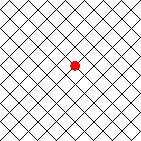
\includegraphics[scale=1.1]{figures/tikz/TFI/site_indices/site_index_a.pdf}
		}
	\end{minipage}	
	\par\medskip
	\begin{minipage}{1.0\textwidth}
		\hspace{20pt}
		\begin{tikzpicture}[scale=1, trim axis left, trim axis right]
			\begin{axis}[xlabel=$t$, ylabel=$\langle\hat{\sigma}_z\rangle$, grid=both, grid style={gray!20}, every axis plot/.append style={very thick}, scale only axis, height=\globalQuenchLargeFieldFigureHeight, width=\globalQuenchLargeFieldFigureWidth, xmin=-0.05, xmax=1.05, ymin=0.5, ymax=1.1]
				%	
				\addplot[color = 5blue1]
				table[x=t_tenpy, y=sz_chi_16, col sep=space]{figures/plots/TFI/global_quench/data/global_quench_g_6.0_tenpy_site_index_4_4_1.txt};
				%\addlegendentry{$\chi= 16$}
				%	
				\addplot[color = 5blue2]
				table[x=t_tenpy, y=sz_chi_32, col sep=space]{figures/plots/TFI/global_quench/data/global_quench_g_6.0_tenpy_site_index_4_4_1.txt};
				%\addlegendentry{$\chi= 32$}
				%	
				\addplot[color = 5blue3]
				table[x=t_tenpy, y=sz_chi_64, col sep=space]{figures/plots/TFI/global_quench/data/global_quench_g_6.0_tenpy_site_index_4_4_1.txt};
				%\addlegendentry{$\chi= 64$}
				%	
				\addplot[color = 5blue4]
				table[x=t_tenpy, y=sz_chi_128, col sep=space]{figures/plots/TFI/global_quench/data/global_quench_g_6.0_tenpy_site_index_4_4_1.txt};
				%\addlegendentry{$\chi= 128$}
				%	
				\addplot[color = 5blue5]
				table[x=t_tenpy, y=sz_chi_256, col sep=space]{figures/plots/TFI/global_quench/data/global_quench_g_6.0_tenpy_site_index_4_4_1.txt};
				%\addlegendentry{$\chi= 256$}
				%
			\end{axis}%
			\begin{axis}[scale only axis, height=\globalQuenchLargeFieldFigureHeight, width=\globalQuenchLargeFieldFigureWidth, every axis plot/.append style={very thick}, xmin=-0.05, xmax=1.05, ymin=0.5, ymax=1.1]
				%	
				\addplot[color = 3red1]
				table[x=t_disoTPS, y=sz_disoTPS_D_2, col sep=space]{figures/plots/TFI/global_quench/data/global_quench_g_6.0_disoTPS_site_index_4_4_1.txt};
				%\addlegendentry{$D = 2$}
				%	
				\addplot[color = 3red2]
				table[x=t_disoTPS, y=sz_disoTPS_D_4, col sep=space]{figures/plots/TFI/global_quench/data/global_quench_g_6.0_disoTPS_site_index_4_4_1.txt};
				%\addlegendentry{$D = 4$}
				%	
				\addplot[color = 3red3]
				table[x=t_disoTPS, y=sz_disoTPS_D_6, col sep=space]{figures/plots/TFI/global_quench/data/global_quench_g_6.0_disoTPS_site_index_4_4_1.txt};
				%\addlegendentry{$D = 5$}
				%
			\end{axis}%
		\end{tikzpicture}%
		\quad
		\raisebox{34.2pt}
		{%
			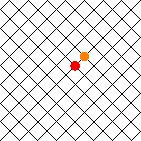
\includegraphics[scale=1.1]{figures/tikz/TFI/site_indices/site_index_b.pdf}
		}
	\end{minipage}
	\par\medskip
	\begin{minipage}{1.0\textwidth}
		\hspace{20pt}
		\begin{tikzpicture}[scale=1, trim axis left, trim axis right]
			\begin{axis}[xlabel=$t$, ylabel=$\langle\hat{\sigma}_z\rangle$, grid=both, grid style={gray!20}, every axis plot/.append style={very thick}, scale only axis, height=\globalQuenchLargeFieldFigureHeight, width=\globalQuenchLargeFieldFigureWidth, xmin=-0.05, xmax=1.05, ymin=0.9, ymax=1.05]
				%	
				\addplot[color = 5blue1]
				table[x=t_tenpy, y=sz_chi_16, col sep=space]{figures/plots/TFI/global_quench/data/global_quench_g_6.0_tenpy_site_index_5_5_0.txt};
				%\addlegendentry{$\chi= 16$}
				%	
				\addplot[color = 5blue2]
				table[x=t_tenpy, y=sz_chi_32, col sep=space]{figures/plots/TFI/global_quench/data/global_quench_g_6.0_tenpy_site_index_5_5_0.txt};
				%\addlegendentry{$\chi= 32$}
				%	
				\addplot[color = 5blue3]
				table[x=t_tenpy, y=sz_chi_64, col sep=space]{figures/plots/TFI/global_quench/data/global_quench_g_6.0_tenpy_site_index_5_5_0.txt};
				%\addlegendentry{$\chi= 64$}
				%	
				\addplot[color = 5blue4]
				table[x=t_tenpy, y=sz_chi_128, col sep=space]{figures/plots/TFI/global_quench/data/global_quench_g_6.0_tenpy_site_index_5_5_0.txt};
				%\addlegendentry{$\chi= 128$}
				%	
				\addplot[color = 5blue5]
				table[x=t_tenpy, y=sz_chi_256, col sep=space]{figures/plots/TFI/global_quench/data/global_quench_g_6.0_tenpy_site_index_5_5_0.txt};
				%\addlegendentry{$\chi= 256$}
				%
			\end{axis}%
			\begin{axis}[scale only axis, height=\globalQuenchLargeFieldFigureHeight, width=\globalQuenchLargeFieldFigureWidth, every axis plot/.append style={very thick}, xmin=-0.05, xmax=1.05, ymin=0.9, ymax=1.05]
				%	
				\addplot[color = 3red1]
				table[x=t_disoTPS, y=sz_disoTPS_D_2, col sep=space]{figures/plots/TFI/global_quench/data/global_quench_g_6.0_disoTPS_site_index_5_5_0.txt};
				%\addlegendentry{$D = 2$}
				%	
				\addplot[color = 3red2]
				table[x=t_disoTPS, y=sz_disoTPS_D_4, col sep=space]{figures/plots/TFI/global_quench/data/global_quench_g_6.0_disoTPS_site_index_5_5_0.txt};
				%\addlegendentry{$D = 4$}
				%	
				\addplot[color = 3red3]
				table[x=t_disoTPS, y=sz_disoTPS_D_6, col sep=space]{figures/plots/TFI/global_quench/data/global_quench_g_6.0_disoTPS_site_index_5_5_0.txt};
				%\addlegendentry{$D = 5$}
				%
			\end{axis}%
		\end{tikzpicture}%
		\quad
		\raisebox{34.2pt}
		{%
			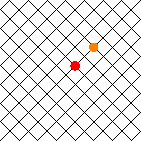
\includegraphics[scale=1.1]{figures/tikz/TFI/site_indices/site_index_c.pdf}
		}
	\end{minipage}
	\caption{In this figure we show the time evolution of the $\langle\hat{\sigma}_z\rangle$ expectation value of a spin in the middle of the lattice and its neighbouring spins. The position of the spins is visualized in the lattice next to the plots. As a model we use the TFI model in the paramagnetic phase with a transverse field of $g = 6$, put on an $8\times8$ diagonal square lattice containing in total $N = 128$ spins. We compute the time evolution once with DMRG on a MPS and once with disoTPS with the parameters given in the text.}
	\label{fig:disoTPS_time_evolution_g_6}
\end{figure}
Finally, we want to test the time evolution in a less challenging regime, for which we used the TFI model at a transverse field of $g = 6$, which is well in the paramagnetic phase. In this regime, entanglement is expected to build up much slower than when simulating at the critical field. We again initialize an all-up-state $|\Psi\rangle = |\uparrow\rangle\otimes\cdots\otimes|\uparrow\rangle$ on the $8\times8$ square lattice but additionally flip a spin in the center. We then compute the time evolution of the $\langle\hat{\sigma}_z\rangle$ expectation value of the flipped center spin and neighbouring spins. The results are shown in figure \figref{fig:disoTPS_time_evolution_g_6}. Note that the DMRG reference simulation converges for much lower bond dimensions $\chi$ compared to figure \figref{fig:disoTPS_time_evolution_g_critical}. We also observe much better agreement of disoTPS TEBD and MPS DMRG.